\chapter{Cats-Effect}

\section{Storia}
Cats-effect è una libreria funzionale per la gestione degli side-effects in Scala, che si basa sui concetti della programmazione funzionale e della teoria delle categorie. Il progetto è stato sviluppato a partire dal 2017 e ha ricevuto una grande attenzione da parte della comunità Scala, diventando uno dei punti di riferimento per la gestione degli side-effects in modo sicuro e componibile. Cats-effect è stato influenzato dalle precedenti libreria come scalaz e monix, ma ha portato nuovi sviluppi in materia di side-effects, come la gestione asincrona e l'astrazione del contesto dell'effetto. Grazie alla sua ampia adozione e alla collaborazione di numerosi sviluppatori, cats-effect è diventato uno strumento fondamentale nella costruzione di applicazioni scalabili e robuste in Scala.

\section{Cos'è Cats-Effect}
Cats Effect è un framework asincrono per la creazione di applicazioni in uno stile puramente funzionale, fornisce uno strumento noto come Monade IO, per catturare e controllare le azioni, chiamate effects, da eseguire in un contesto tipizzato con supporto alla concorrenza e al coordinamento. Gli effects possono essere asincroni (callback-driven) o sincroni (restituiscono direttamente i valori). Cats Effect definisce un insieme di typeclass che definiscono un sistema puramente funzionale.

\noindent Ancora più importante è il fatto che: Cats Effect definisce un insieme di typeclasses che definiscono cosa significa essere un sistema di runtime puramente funzionale. Queste astrazioni alimentano un ecosistema fiorente costituito da framework di streaming, livelli di database JDBC, server e client HTTP, client asincroni per sistemi come Redis e MongoDB e molto altro ancora! Inoltre, è possibile sfruttare queste astrazioni all'interno della propria applicazione per sbloccare potenti funzionalità con poche o nessuna modifica del codice, ad esempio risolvere problemi come l'iniezione di dipendenze, canali di errore multipli, stato condiviso tra moduli, tracciamento e altro ancora.

Cats-Effect è quello che viene chiamato un asyncronous framework, ovvero un framework che ti permette di scrivere applicazioni che possono/devono essere asincrone o che traggono un vantaggio dall'effettuare alcune operazioni concorrentemente.  Di framework di programmazione asincrona ne esistono diversi, in diversi linguaggi, su JVM abbiamo \href{https://github.com/ReactiveX/RxJava}{RxJava}, \href{https://vertx.io/}{Vert.x}, \href{https://netty.io/}{Netty} e \href{https://akka.io/}{Akka}, mentre in Rust abbiamo ad esempio \href{https://tokio.rs/}{Tokio} . Alcuni di essi, ad esempio Akka e Netty sono implementati usando le ThreadPools, ovvero insiemi di Thread a cui posso "inviare" una computazione ed aspettarmi che uno di quei thread eventually esegua quel task e che me ne restituisca il risultato. Cats-effect è un runtime che nasce la gestione di Green Thread (thread che nasce nativamente sulla VM e non sul sistema operativo sottostante), che su JVM è stato di recente implementato grazie a progetto Loom (Loom vuol dire telaio, per correlazione con le fibre), concetto che in rust è stato implementato da tokio e da tokio è stato copiato in Cats-Effect. Entriamo più nel dettaglio del framework esplorandone i sui costrutti. 

\section{Side Effect}
Per definizione una funzione contiene un side-effect se non gode della trasparenza referenziale. Vale a dire una funzione che quando riceve lo stesso parametro in input, restituisce sempre lo stesso valore in output. Quindi una funziona ha un side-effect quando ad esempio modifica una variabile al di fuori del proprio livello di scoping, quando modifica uno dei suoi argomenti, quando scrive su file o quando invoca altre funzioni con side-effects.

\section{Elementi Principali}
Nelle seguenti sezioni definiamo quelli che sono i principali elementi che costituiscono la libreria.
\subsection{IO}
Un IO in Cats-Effect è una struttura dati che rappresenta una descrizione di una computazione sincrona o asincrona con side-effects. Un valore di tipo IO[A] è una computazione che, se valutata, può eseguire side effect prima di restituire un valore di tipo A. I valori IO sono puri e immutabili e quindi preservano la trasparenza funzionale.
\begin{minted}{scala}
val num: IO[Int] = IO.pure(1)  //caso in cui non ho side effect
\end{minted}
\begin{minted}{scala}
val delayIO: IO[Int] = IO.delay({ 
    println("Hello World!")
    10
})  //viene valuta quando viene chiamata

//può essere anche scritta come: 

val v1DelayIO: IO[Int] = IO {  //sfruttando apply
    println("Hello World!")
    10
} 
\end{minted}
Ma uno dei aspetti più importanti di IO è che consente lo stile monadico. Infatti IO è anche una Monade in dove ogni riga viene concatenata alla successiva usando l'operatore flatMap, il cui nome in haskell é bind e in typescript chain e spesso viene indicato con >>=, ad esempio:

\begin{minted}{scala}
val p: Person = ???
def getName(person:Person): IO[String] = ???
def getSurname(person:Person): IO[String] = ???

//Possiamo definire la concatenazione di nome e cognome come:

val completeName: IO[String] = getName(p).flatMap(name => getSurname(p)
                                                     .map(surname => s"$name $surname"))
    
\end{minted}

\noindent Si noti che questo approccio può essere riscritto utilizzando la for-comprehension come segue:
\begin{minted}{scala}

val completeName: IO[String] = 
  for {
    name    <- getName(p)
    surname <- getSurname(p)
  } yield s"$name $surname"
    
\end{minted}


\subsection{Fibers}
Un fiber è l'astrazione di un Green Thread, che su JVM è stato di recente implementato grazie a progetto Loom (Loom vuol dire telaio, per correlazione con le fibre), concetto che in rust è stato implementato da tokio e da tokio è stato copiato in Cats-Effect. Le fibre non sono altro che una implementazione delle API di green thread. L'idea alla base è basata sul fatto che che sono dei thread che puoi istanziare in gran numero e che vengono gestiti da un sistema di schedulazione. Quindi si pongono come un livello di astrazione superiore a quello dei thread e gestiscono le così dette ThreadPools, possiamo paragonarli agli Executors in Java. Un'entità (nel caso di cats-effect il suo runtime) alloca una thread pool (la cui dimensione e tipologia sono scelte secondo una logica ottimale presente nella libreria) che viene utilizzata come se ogni singolo thread fosse una cpu e su questi thread, lo schedulatore presente nel runtime di cats-effect, schedula i "pezzi di programma" o azioni da eseguire. Che forma hanno questi pezzi di programma? Sono degli IO, infatti un fiber esegue un’azione F che è tipicamente un’istanza IO.
I thread che necessita il runtime di cats-effect sono vari e si occupano principalmente di:
\begin{itemize}
    \item gestire i comportamenti e elementi interni, come lo schedulatore;
    \item gestire i IO compute intensive;
    \item gestire le operazioni bloccanti (come la scrittura su file e le comunicazioni di rete). Il numero di thread in questa thread pool è circa (numero di CPU -1), in modo da gestire al massimo n-1 task bloccanti su n-1 cpu e di riservarne una per lo scheduler.
\end{itemize}
Gran parte di questa complessità è mascherata dalla libreria e di fatto la libreria ti permette di usare il suo runtime in modo invisibile, è sufficiente creare degli IO e usare flatmap. I fibers sono molto leggeri rispetto ai thread quindi si possono generare milioni di fibers senza influire sulle prestazioni.

\section{Stile monadico}
Nel 1991 Eugenio Moggi, professore di Informatica all'Università degli Studi di Genova, pubblicò un saggio, nel quale considerava l'utilizzo della monade, attraverso la semantica del Lambda calcolo, per gestire gli effetti collaterali, gli input e gli output, le eccezioni ed altro. Le monadi sono un'entità matematica che rispetta determinate leggi, chiamate leggi monadiche, e nella programmazione funzionale le si utilizza molto. Questa pubblicazione ha influito sul lavoro di molti informatici, tra i quali Simon Peyton Jones, il quale, poi le implementerà nel linguaggio puramente funzionale Haskell (al posto di utilizzare delle lazy-list per gestire l'IO). Come abbiamo visto Nella programmazione funzionale, una monade è una struttura che esprime una classe di computazioni concatenabili. Con l'ausilio di questa struttura, è possibile compiere, anche nei linguaggi puramente funzionali, operazioni in sequenza, un po' come avviene nei linguaggi imperativi o procedurali. Infatti, possono essere espresse, con l'ausilio delle monadi, fenomeni come gli effetti collaterali, l'IO, gestione dell'eccezioni.

\noindent In Haskell, la classe Monad viene espressa come segue:
\begin{minted}{haskell}
class Monad m where
  (>>=)  :: m a    -> (a  -> m b) -> m b
  (>>)   :: m a    -> m b -> m b            -- non strettamente necessaria
  return :: a      -> m a
  fail   :: String -> m a                   -- non strettamente necessaria
\end{minted}

Eugenio Moggi  si accorse che una struttura della teoria delle categorie, la monade era molto efficace nel descrivere catene di programmi che potrebbero non terminare e con la caratteristica che il primo programma che si rompe rompe anche la catena questo perchè le monadi sono un'entità matematica che rispetta determinate leggi, chiamate leggi monadiche, scrivere delle strutture dati monadiche che rispettano queste leggi permette di scrivere programmi in stile monadico, che utilizzando gli operatori che tutte le monadi hanno a disposizione per combinare diversi programmi tra di loro o per applicare funzioni ai valori contenuti al loro interno. 

Una diretta conseguenza è l'importanza che assume la monade IO di cats-effect che consente di: 

\begin{itemize}
    \item Controllare l'esecuzione di programmi asincroni, che possono anche produrre side effects, utilizzando un’interfaccia pulita.
    \item Gestire applicazioni altamente simultanee concorrenti, Cats-effect non è formidabile nel gestire programmi compute intensive, ma eccelle nel gestire programmi che fanno molto I/O di rete o scrittura su più files.
    \item  La concorrenza in IO  è costruita con le fibers: un'implementazione dei green thread, come le couroutine sospendibili, gestite a runtime. 
    \item Gestire i cicli di vita delle risorse e garantire che le risorse siano allocate e rilasciate in modo sicuro anche in presenza di eccezioni e interruzioni. La gestione delle risorse è più complesso in applicazioni concorrenti; un piccolo bug potrebbe causare una perdita di dati o persino un deadlock bloccando il sistema.
    \item  scrivere programmi semplici che possono essere composti per formare programmi più complessi, pur mantenendo la capacità di ragionare sul comportamento e sulla complessità. Questo è possibile grazie al fatto che IO è stato costruito come una monade, e quindi puoi usare tutti gli operatori e le proprietà di una monade.
\end{itemize}


\section{TypeClasses}
La gerarchia delle classi di tipo all'interno di Cats Effect definisce, fondamentalmente, cosa significa essere un effetto funzionale. Questo si traduce nel dire, rispettiamo una serie di regole(laws) che ci dicono cosa significa essere un numero o cosa significa avere un metodo flatMap. Lo schema seguente mostra la gerarchia di type classes di Cats Effects.

\begin{figure}[H]
    \centering
    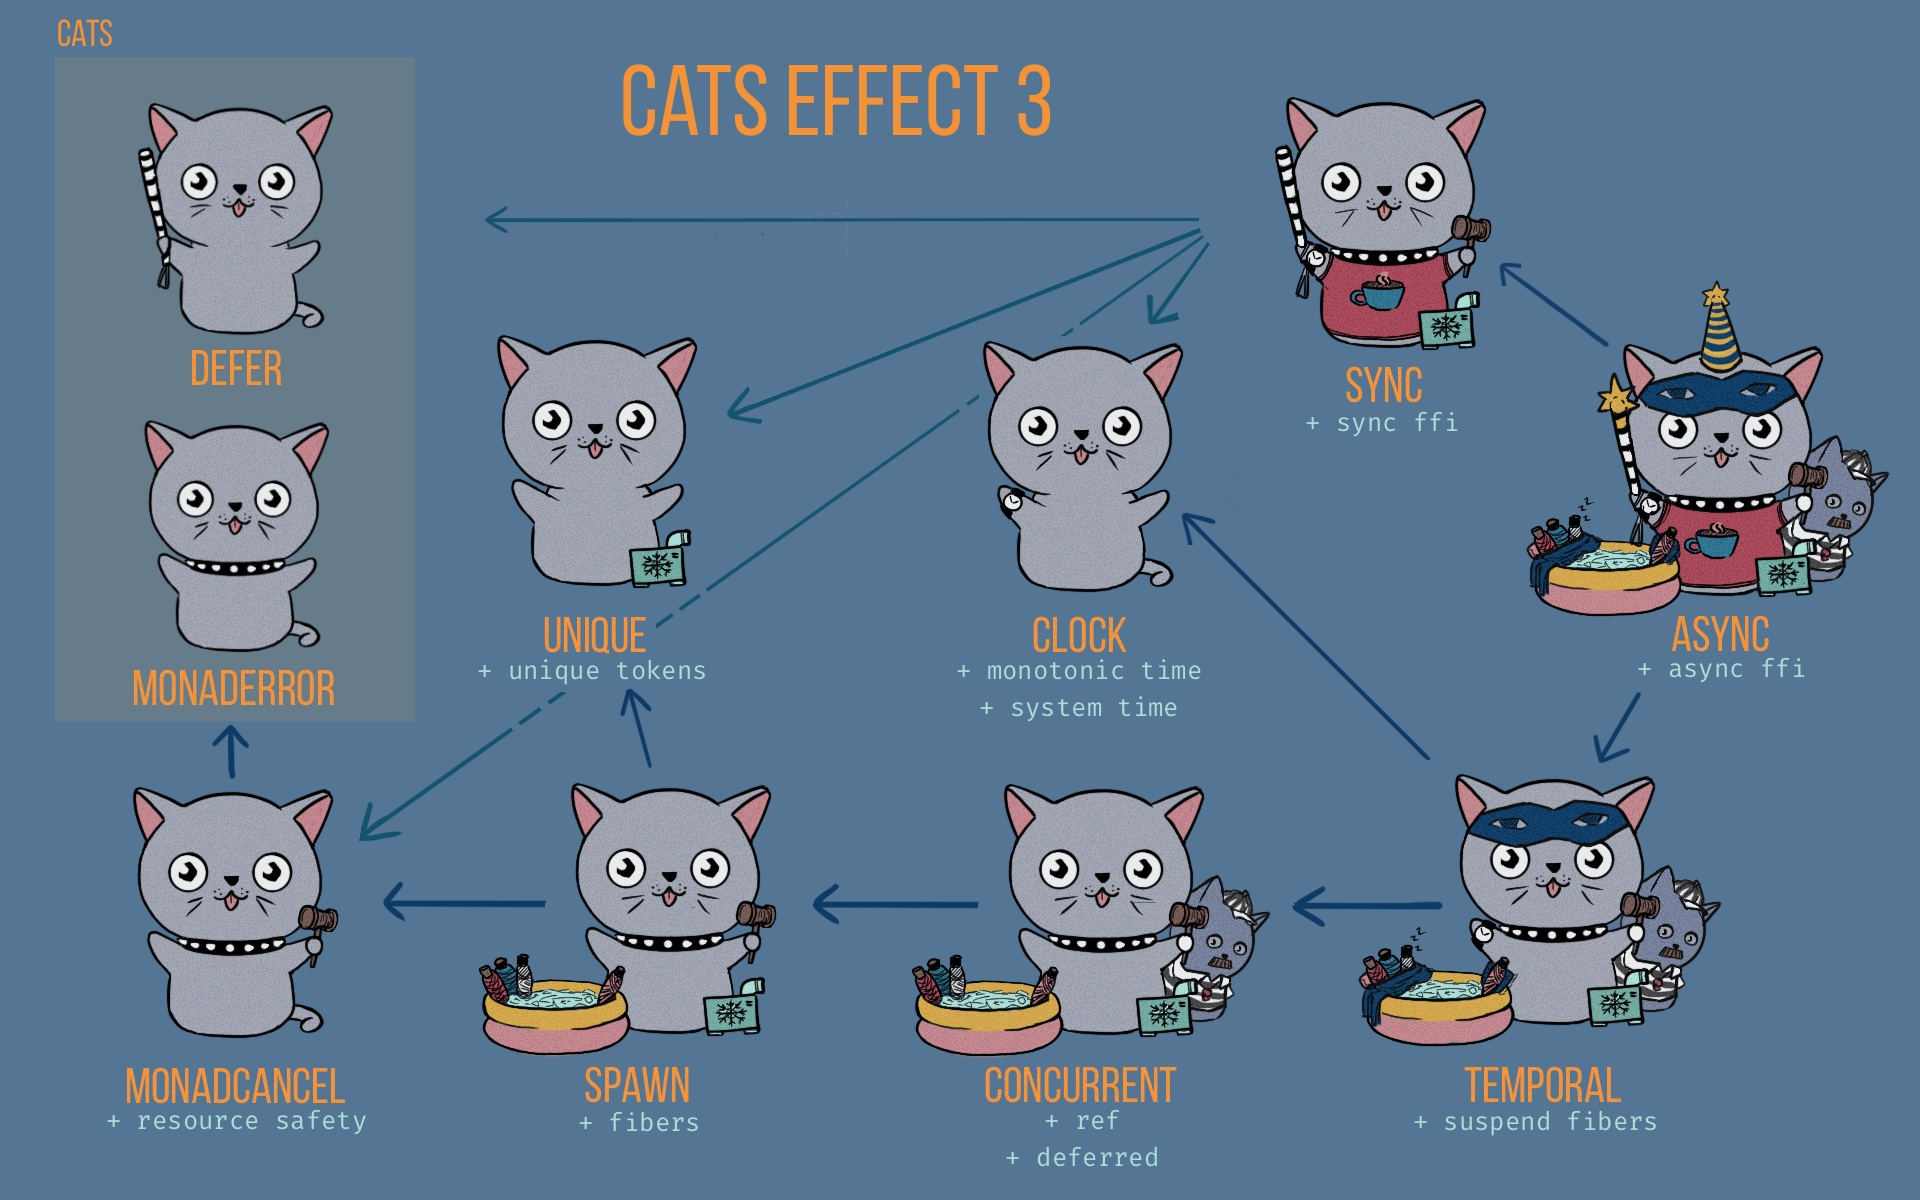
\includegraphics[scale=0.2]{img/hierarchy-impure.jpeg}
    \caption{Gerarchia type classes in Cats-effect 3.}
    \label{fig: Gerarchia type classes in Cats-effect 3}
\end{figure}

\noindent In generale, le regole per gli effetti funzionali possono essere suddivise nelle seguenti categorie elencate in ordine di potenza crescente :

\begin{itemize}
    \item Sicurezza e interruzione/cancellazione nell'utilizzo delle risorse;
    \item Valutazione parallela di side-effects;
    \item Condivisione dello stato tra processi paralleli;
    \item Interazioni con il tempo;
    \item Acquisizione sicura dei side-effect che restituiscono valore;
    \item  Acquisizione sicura dei side-effects che hanno una callback;
\end{itemize}

\noindent Alcune funzionalità sono assunte da Cats Effect ma definite all'interno di Cats e i suoi moduli. Tali capacità sono le seguenti:
\begin{itemize}
    \item Trasformare il valore all’interno di un effetto mappandolo sopra di esso.
    \item Inserire un valore in un effetto.
    \item Comporre più calcoli efficaci insieme in sequenza, in modo tale che ognuno dipenda dal precedente.
    \item Generare e gestire gli errori.
\end{itemize}

\noindent Nel loro insieme, tutte queste capacità definiscono cosa significa essere un effetto. Ciò ti consente di comprendere e rifattorizzare il tuo codice in base a regole e astrazioni, piuttosto che dover pensare a ogni possibile dettaglio di implementazione e caso d'uso. Inoltre, consente a te e ad altri di scrivere codice molto generico che si compone insieme facendo ipotesi minime. Questa è la base dell'ecosistema Cats Effect. Di seguito vengono mostrate le typeclasses di Cats-effect con le relative API insieme ad esempi di utilizzo anche complessi.

\subsection{MonadCancel}
Tipicamente un fiber termina con tre stati sottotipi di Outcome che sono Succeeded, Errored e Canceled. 

\begin{minted}{scala}
sealed trait Outcome[F[_], E, A]
final case class Succeeded[F[_], E, A](fa: F[A]) extends Outcome[F, E, A]
final case class Errored[F[_], E, A](e: E) extends Outcome[F, E, A]
final case class Canceled[F[_], E, A]() extends Outcome[F, E, A]    
\end{minted}

\noindent Ciò significa che quando si scrive codice sicuro per le risorse, dobbiamo preoccuparci dell'annullamento e delle eccezioni. La typeclass MonadCancel risolve questo problema estendendo MonadError(definito in Cats) per fornire la capacità di garantire il funzionamento dei finalizzatori quando una fibra viene cancellata. Usandolo, possiamo definire effetti che acquisiscono e rilasciano risorse in modo sicuro come ad esempio \textbf{bracket} che è l'equivalente di programmazione funzionale di try/finally:

\begin{minted}{scala}
    openFile.bracket(fis => readFromFile(fis))(fis => closeFile(fis))
\end{minted}

\noindent Bracket fa si che se viene eseguito openFile verrà di certo eseguito closeFile. Ciò accade anche se readFromFile produce un
errore o viene interrotto da qualche altro fiber. Inoltre openFile è atomico: o non viene valutato per niente o viene valutato 
completamente permettendo di fare calcoli complessi senza temere che qualcosa di esterno si intrometta. Oltre a bracket, MonadCancel fornisce anche un'operazione di livello inferiore, \textbf{uncancelable} che consente di eseguire azioni estremamente complesse e sensibili all'annullamento in modo sicuro e componibile.. Si pensi ad un blocco di codice protetto da un Semaforo, a cui si deve garantire la mutua esclusione ci si troverebbe in un problema legato all’acquisizione del Semaforo, che è una risorsa, che può anche comportare il blocco del fiber, e quindi potrebbe essere necessario interromperlo dall’esterno. In generale, vorremmo che l’acquisizione delle risorse sia non interrompibile, ma in questo caso particolare si deve consentire l’interruzione, altrimenti potrebbe finire per bloccare la JVM e entrare in uno stato di deadlock del sistema. L'esempio seguente mostra come Uncancelable fornisce una soluzione per raggiungere questo obiettivo:

\begin{minted}{scala}
    def guarded[F[_], R, A, E](
    s: Semaphore[F],
    alloc: F[R])(
    use: R => F[A])(
    release: R => F[Unit])(
    implicit F: MonadCancel[F, E])
    : F[A] =
  F uncancelable { poll =>
    for {
      r <- alloc //acquisizione della risorsa  r
      // viene utilizzato il metodo poll per eseguire l'operazione di acquisizione
      // del semaforo s in modo cancellabile
      //nel caso in cui viene interrotta viene effettuata la releaseAll per il
      //rilascio della risorsa r
      _ <- poll(s.acquire).onCancel(release(r)) 
      releaseAll = s.release >> release(r)
        // guarantee fa si che il rilascio sia sempre garantito, anche in caso 
        //di eccezioni o interruzioni durante l'utilizzo della risorsa.
      a <- poll(use(r)).guarantee(releaseAll)
    } yield a
  }
\end{minted}

\noindent Abbiamo che l'esecuzione è avvolta in uncancelable, il che significa che non dobbiamo preoccuparci che altre fibre ci interrompano nel mezzo di ciascuna di queste azioni. La primissima azione che eseguiamo è alloc, che alloca un valore di tipo R. Una volta che questo è stato completato con successo, tentiamo di acquisire il  Semaphore. Se un altro fiber ha già acquisito il
semaforo, il fiber corrente potrebbe bloccarsi per un po'. Vogliamo che altre fibre siano in grado di interrompere questo blocco, quindi avvolgiamo l'acquisizione in poll che riabilita l’interruzione all’interno di uncancelable per tutto ciò che avvolge. Se l’acquisizione del semaforo viene interrotta, ci si vuole assicurare di rilasciare la risorsa r utilizzando onCancel.  Infine si passa all’invocazione dell’azione use(r) che indipendentemente dal suo risultato (successed, canceled, errored) fa si che venga eseguita la releaseAll che che rilascia l’acquisizione del semaforo e della risorsa.

Un altra particolarità di MonadCancel è la capacità di auto-annullarsi. Per esempio:
\begin{minted}{scala}
    MonadCancel[F].canceled >> fa
\end{minted}

\noindent Quanto sopra si tradurrà in un auto-annullamento e fa non verrà mai eseguita, a condizione che non sia racchiusa in un blocco uncancelable.

\subsection{Spawn}
Questa typeclass fornisce un’astrazione simile a Thread, che può essere implementata per computazioni parallele. Come già detto in precedenza i fibers sono Green thread, è infatti possibile averne anche milioni su un’unica macchina. Immaginiamo ad esempio, un'applicazione che implementa un microservizio probabilmente desidererebbe almeno un'azione simultanea per richiesta in un dato momento, ma se il numero di azioni simultanee è limitato al numero di thread disponibili (che a sua volta è limitato al numero di processori disponibili!), è improbabile che il servizio si ridimensioni particolarmente bene; ad oggi le applicazioni risolvono questo problema attraverso l'uso di thread pool e ad e altre tecniche manuali che sebbene funzionino ragionevolmente bene, sono abbastanza facili da sbagliare e molto limitate in termini di funzionalità che si può costruire su di esse. È necessaria un'astrazione migliore, che consenta al framework e al codice utente di generare semplicemente azioni semantiche secondo necessità (ad esempio per gestire una richiesta in arrivo), mentre il runtime sottostante si occupa della mappatura di tali azioni a thread del kernel reali in un moda ottimale. Prendiamo ad esempio un server che accetta delle connessioni:

\begin{minted}{scala}
import cats.effect.{MonadCancel, Spawn}
import cats.effect.syntax.all._
import cats.syntax.all._

trait Server[F[_]] {
  def accept: F[Connection[F]]
}

trait Connection[F[_]] {
  def read: F[Array[Byte]]
  def write(bytes: Array[Byte]): F[Unit]
  def close: F[Unit]
}

def endpoint[F[_]: Spawn](
    server: Server[F])(
    body: Array[Byte] => F[Array[Byte]])
    : F[Unit] = {

  def handle(conn: Connection[F]): F[Unit] =
    for {
      request <- conn.read
      response <- body(request)
      _ <- conn.write(response)
    } yield ()

  val handler = MonadCancel[F] uncancelable { poll =>
    poll(server.accept) flatMap { conn =>
      handle(conn).guarantee(conn.close).start
    }
  }

  handler.foreverM // Gestisce le connessioni in maniera continua
}
\end{minted}

Per l’handler si utilizza uncancelable per evitare perdite di risorse tra quando si ottiene la connessione a quando si imposta la gestione delle risorse. Per ogni connessione
la si gestisce con la funzione \textbf{handle} e indipendentemente dall’esito la si chiude, successivamente si utilizza start per creare un nuovo fiber per ogni richiesta di connessione che arriva.

\subsubsection{Cancelation}
Il vantaggio di utilizzare i fibers oltre ad essere leggeri è che a differenza dei thread della JVM sono interrompibili. Ciò significa che è possiile utilizzare \textbf{cancel} su un fiber in esecuzione per avviare il processo di ripulitura delle risorse allocate e fermarsi. Possiamo verificare questa proprietà con una monade IO come segue:
\begin{minted}{scala}
for {
  target <- IO.println("Catch me if you can!").foreverM.start
  _ <- IO.sleep(1.second)
  _ <- target.cancel
} yield ()
\end{minted}

Il comportamento di questo codice è il seguente: 
\begin{itemize}
    \item la fibra targer stamperà un numero non deterministico di volte la frase "Catch me if you can!"
    \item quando la fibra principale smette di dormire per un secondo la fibra targer viene annullata. Tecnicamente, l'annullamento potrebbe non riflettersi istantaneamente nella fibra target ma appena la fibra target viene cancellata/annullata, la stampa viene interrotta e il programma termina. Utilizzando Thread è impossibile replicare questo esempio senza costruire il proprio meccanismo per l’interruzione. Con fiber per`è  già tutto gestito dalla typeclass Spawn.

\end{itemize}

\subsubsection{Joining}
Di solito quando si eseguono delle operazioni in parallelo si desidera attendere che finiscano, accettare i risultati e andare avanti. L'astrazione dei Thread in Java ha l'operatore join, nelle fibre abbiamo qualcosa di simile definito come segue:
\begin{minted}{scala}
def both[F[_]: Spawn, A, B](fa: F[A], fb: F[B]): F[(A, B)] =
  for {
    fiberA <- fa.start
    fiberB <- fb.start

    a <- fiberA.joinWithNever
    b <- fiberB.joinWithNever
  } yield (a, b)
\end{minted}
\noindent Il metodo \textbf{joinWithNever} è un metodo semplificato basato su join, che è molto più generale. In particolare, il metodo \textbf{Fiber\#join} restituisce \textbf{F[Outcome[F, E, A]]} (dove E è il tipo di errore per F). Outcome ha la seguente forma:
\begin{itemize}
    \item Succeeded: contiene un valore di tipo F[A].
    \item Errored: contiene un valore di tipo E solitamente Throwable.
    \item Canceled: non contiene niente.
\end{itemize}
\noindent Questi rappresentano i tre possibili stati di terminazione per un fiber e c’è la possibilità di reagire a ciascuno in modo diverso. Ad esempio:
\begin{minted}{scala}
fiber.join flatMap {
    /* In caso di successo */
    case Outcome.Succeeded(fa) =>
        fa
    /* In caso di errore */
    case Outcome.Errored(e) => ???
    /* Quando il fiber viene interrotto */
    case Outcome.Canceled() => ???
}
    
\end{minted}

\noindent Il seguente codice è un implementazione di quanto descritto sopra che stampa per 3 secondi Hello I am Fiber A e Hello I am Fiber B e in seguito racchiude un intero in IO: 
\begin{minted}{scala}
for {
    fiberA <- (IO.println("Hello I am Fiber A").foreverM.timeoutTo(3.seconds, IO.unit)
        >> IO.pure(1)).start
    fiberB <- (IO.println("Hello I am Fiber B").foreverM.timeoutTo(3.seconds, IO.unit)
        >> IO.pure(1)).start
        
    /* Attendo il completamento */
    a <- fiberA.joinWithNever
    b <- fiberB.join flatMap {
        case Outcome.Succeeded(fb) => fb
        case Outcome.Errored(e) => MonadError[IO, Throwable].raiseError(e)
        /* Nel caso in cui il fiber figlio venga interrotto, si cerca di
        interrompere l'attuale fiber, se non è possibile si cade in deadlock */
        case Outcome.Canceled() => MonadCancel[IO].canceled >> Spawn[IO].never
    }
    
    _ <- IO.println(s"a: $a, b: $b")
} yield (a, b)
    
\end{minted}

\subsection{Unique}
Unique è una typeclass che genera token univoci. Il suo uso avviene principalmente a basso livello, perchè tipicamente è indatta ad identificare entità a livello di logica di applicazione come UUID. Si definisce come: 
\begin{minted}{scala}

trait Unique[F[_]] {
  def unique: F[Unique.Token]
}
\end{minted}

L'unicità è garantita dal confronto di uguaglianza tra istanze Unique.Token che non sono serializzabili o convertibili attualmente allocate. Se un token viene liberato dal Garbage Collector quel token può essere
riallocato a seguito di una nuova chiamata a unique. La garanzia di unicità è  presente solo all’interno di una singola JVM. Entramble le typeclasses Sync[F] che Spawn[F] estendono Unique[F] poichè entrambe possono creare valori univoci tramite delay e start (i fibers sono sempre unici). 
\begin{minted}{scala}
    delay(new Unique.Token())
    start(new Unique.Token())
\end{minted}

\subsection{Clock}
Clock è una typeclass che fornisce un sistema analogo a System.nanoTime() e System.currentTimeMillis() per la gestione del tempo. E' definito come:
\begin{minted}{scala}
trait Clock[F[_]] {
  def monotonic: F[FiniteDuration]
  def realTime: F[FiniteDuration]

}
\end{minted}

Il seguente codice mostra un uso di realTime di clock per calcolare il tempo trascorso da un dato momento ad un altro:

\begin{minted}{scala}
for {
    start <- Clock[IO].realTime
    _ <- IO.sleep(3.seconds)
    end <- Clock[IO].realTime
    _ <- IO.println(end - start) // Tempo trascorso in millisecondi => 3000
} yield ()
    
\end{minted}

\subsection{Concurrent}
\subsection{Temporal}
\subsection{Sync}
\subsection{Async}